

\documentclass[]{article}
\usepackage{graphicx}
\usepackage{amsmath}
\usepackage{amssymb}
\usepackage{amsfonts}
\usepackage{fancyhdr}
\usepackage[headheight=65pt,tmargin=150pt,headsep=95pt]{geometry}
\usepackage{ragged2e}
\usepackage{array}
\usepackage{tabularx}
%list of images


\graphicspath{{./images/}}

\pagestyle{myheadings}
\markright{Extra Solar Lab Report\hfill 2663452m\hfill 16/1/2023\hfill}

\title{\textbf{Identifying Extra Solar Planets and their Key Features using 
the Doppler Wobble and Planetary Transits Methods}}
\author{2663452m (University of Glasgow)}
\date{16/1/2023}






\begin{document}
\maketitle

\begin{abstract}
This is the abstract

\end{abstract}
\newpage


% All relevant sections for Method 1 (Doppler Wobble)

\twocolumn
\section*{Introduction and Background}

\section*{The Doppler Wobble Method of extra-solar planets}
\par
For the analysis on data of two stars and the existence of an extra-solar planets 
around them, the doppler wobble method was used. This method is based on measuring the 
radial velocity of the stars (HD-28185 and HD-73256) as they move towards and away from 
the observer. Thus
producing a doppler shift in the light emitted from the stars, that can be used to 
determine the velocity of the stars in the plane of the observer's line of sight. 
\par
To determine the radial velocity, observations were made of the stars on different
Julian dates, recording the wavelength of light emitted as well as the observed intensity 
of the light. The radial velocity of the stars can then be calculated using the doppler
shifted wavelength and intensity, as provided in the Python Library.$^1$ 
\begin{equation}\label{eq:wavelength doppler}\lambda_{obs} = \lambda_{emit}{(1+v/c)}
\end{equation}

\begin{equation}\label{eq:intensity doppler}I_{obs} = \frac{I_{emit}}{(1+v/c)}
\end{equation}
where $\lambda_{obs}$ is the observed wavelength, $\lambda_{emit}$ is the 
emitted wavelength, $I_{obs}$ is the observed intensity, $I_{emit}$ is the emitted 
intensity, $v$ is the radial velocity of the stars and $c$ is the speed of light.
From this it was possible to calculate the radial velocity of each star on each date.
This was done using the Python SCIPY library.$^2$ An uncertainty in the radial velocity
was assigned to each date of each star of $\pm 15 ms^-1$.$^1$
\par

\begin{figure}[h]
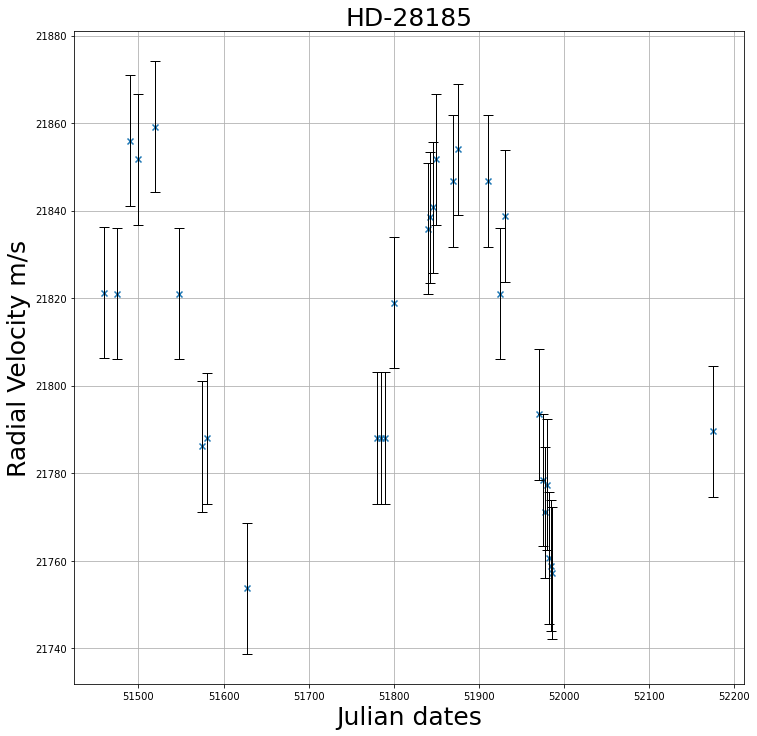
\includegraphics[width=6cm]{images/HD-28185_init.png}
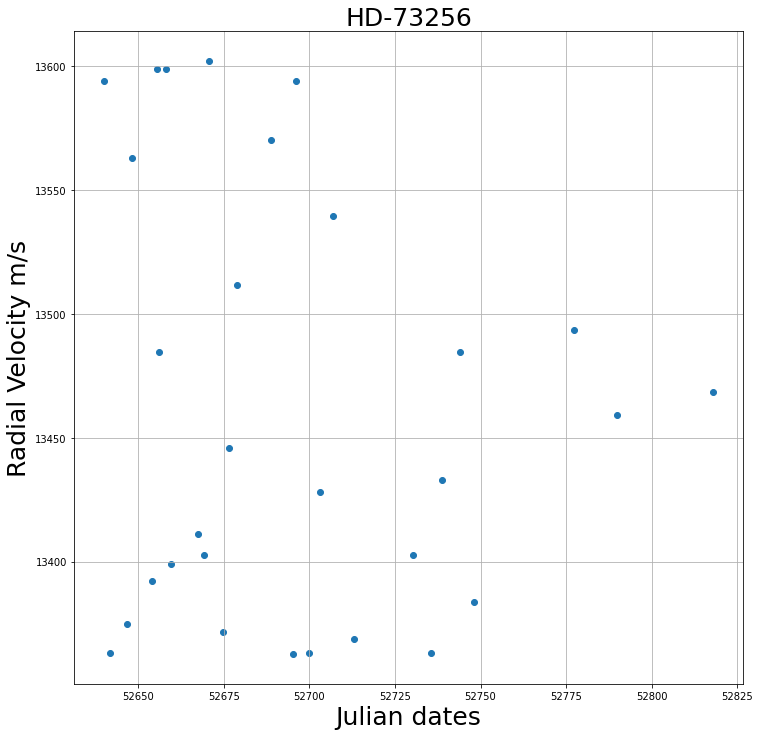
\includegraphics[width=6cm]{images/HD-73256_init.png}
\caption{Radial velocity of HD-28185 and HD-73256 as a function of time (Julian Date)}
\label{fig:HD-_init}
\end{figure}

When plotting the radial velocity as a function of time, as seen in figure 1, it was
possible to see that there was a periodic sinusoidal pattern in the data, however, 
it was not very accurate as the time between observations varyed.
To correctly plot the radial velocity of the stars over time it was neccessary 
to calculate the phase of each star through the period of the orbit. In this experiment
the phase is defined as the fraction of the orbital period that has elapsed.
The radial velocity of the stars (HD-28185 and HD-73256) as a function of phase 
was then plotted, as seen in figure 2. This allowed for a more accurate representation
of the radial velocity of the stars as a function of time, as the time between 
observations was more consistent.
\par
\newpage

\begin{figure}[h]
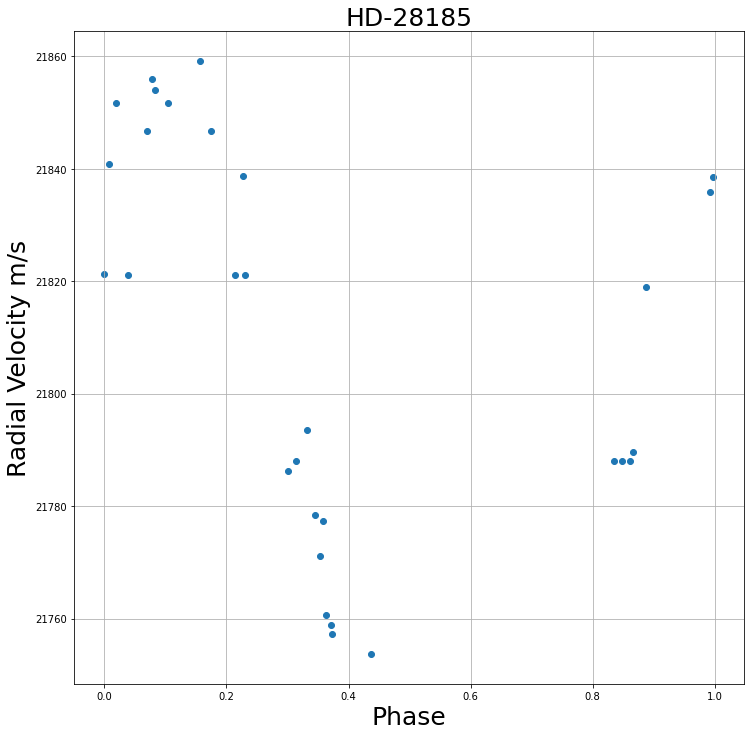
\includegraphics[width=6cm]{images/HD-28185_phase.png}
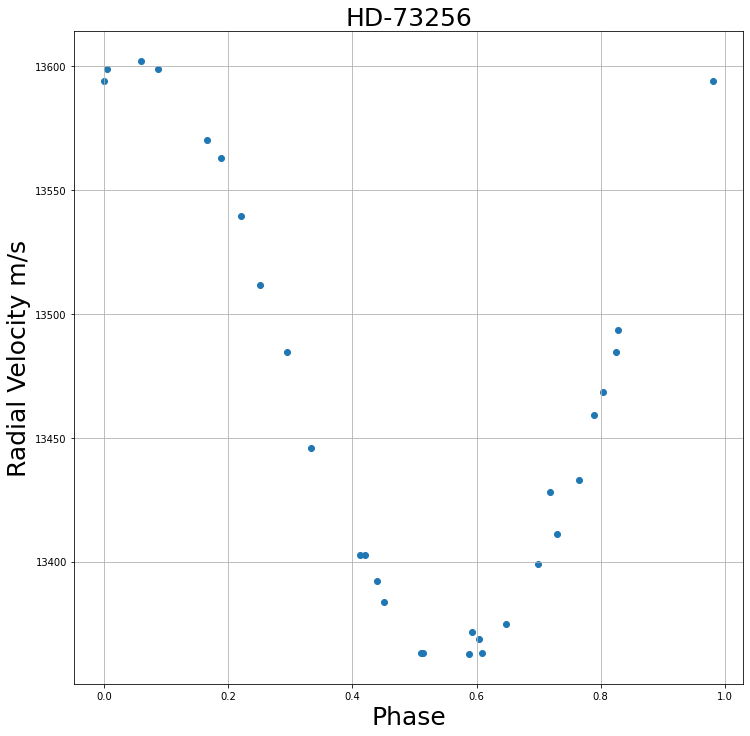
\includegraphics[width=6cm]{images/HD-73256_phase.png}
\caption{Radial velocity of HD-28185 and HD-73256 as a function of phase}
\label{fig:HD-_phase}
\end{figure}

Now that there was a clear correlation between the radial velocity of the stars and
time, it was possible to calculate characteristics about the extra-solar planets in 
orbit around the stars (HD-28185 and HD-73256) using %equation 2 from lab script. 
By using the data calculated so far in this report it was possible to now calculate 
the mean radial velocity $v_{mean} $, the amplitude of the radial velocity curve
 $v_{s}$ and the 
phase when the radial velocity curve is at a maximum $\phi_{max}$ of the stars.
As well as the associated covariance matrix uncertainties for each of these values.
\par
For the stars (HD-28185 and HD-73256) the values obtained for $v_{mean}$, $v_{s}$ 
and $\phi_{max}$ 


\begin{table}[]
    \begin{tabularx}{5cm}{|c|c|c|c|}
    \hline
    Star     & \begin{tabularx}[c]{@{}c@{}}$\\ v_{mean} $\end{tabular}                     & \begin{tabularx}[c]{@{}c@{}}$\\ v_{s}$\end{tabular}                              & \begin{tabularx}[c]{@{}c@{}}$\\  \phi_{max}$\end{tabular}                  \\ \hline
    HD-28185 & \begin{tabularx}[c]{@{}c@{}}$\\ 2.18\times10^4 \pm4.00ms^{-1}$\end{tabular} & \begin{tabularx}[c]{@{}c@{}}$67.6\\ \pm\\ 6.16\\ ms^{-\\ 1\\ } \\ $\end{tabular} & \begin{tabularx}[c]{@{}c@{}}$\\  8.59\times10^{-2} \pm 0.01 $\end{tabular} \\ \hline
    HD-73256 & $1.35\times10^4\pm2.80ms^{-1}$                                             & $1,20\times10^2\pm3.92ms^{-1}$                                                  & $5.73\times10^{-2}\pm0.01$                                                \\ \hline
    \end{tabular}
\end{table}





\section*{Method}
For the Doppler Wobble method it was first necessary to 
import all the data provided into a directory that could be 
accessed by the code source files. From here it was possible to start
writing the Python script that would take the data and produce the required 
outputs as outlined in the aims above.




\section*{Results}
For doppler wobble method 1.1 result is graph. \par
1.2 radial velocity of both stars on all dates\par
1.3 plot radial velocity as a function of time, calculate the phase
of each star and plot the radial velocity as a function of phase\par
1.4 calculate values of v$_{mean}$ v$_{s}$ and $\phi_{max}$ and determine errors,
for both stars\par
1.5 calculate the mass of each planet and the semi-major axis of each planet 
with errors\par



\section*{Analysis}





% All relevant sections for Planetary transits method
\newpage
\section*{Introduction and Background}

\section*{Aims}

Obtain a phase-folded photometric light curve for a star with a transiting 
planetary companion. Use this to estimate the radius and orbital semi-major 
axis of the planet
Apply the method of least-squares to estimate mean apparent magnitudes 
during the transit and non-transit phase. Hence estimate the radius of the planet.$^1$


\section*{Method}

\section*{Results}

\section*{Analysis}


\section*{Conclusion}

\section*{References}
\end{document}